\documentclass[11pt]{article}
\usepackage[margin=1in]{geometry}
\usepackage{booktabs}
\usepackage{xcolor}
\usepackage{amsmath}
\usepackage{float}
\usepackage{graphicx}
\usepackage{hyperref}
\hypersetup{colorlinks=true, linkcolor=blue!60!black}

\newcommand{\win}[1]{\textcolor{green!50!black}{\textbf{#1}}}
\newcommand{\bad}[1]{\textcolor{red!70!black}{#1}}

\title{Random Network Routing Evaluation}
\author{Autonomous Networks Research Group (ANRG)\\University of Southern California}
\date{}
\begin{document}
\maketitle
\tableofcontents
\newpage

\section{Evaluation Setup}

Does the relative performance ranking of HEFT, HEFT-1, and HEFT-2 hold
on random graphs?  We place \textbf{50 nodes} uniformly at random in an
$L\times L$ square and create bidirectional links between all pairs within
$R=80$\,m.  Varying $L$ controls network density.

\begin{table}[H]\centering
\begin{tabular}{ll}\toprule
\textbf{Parameter} & \textbf{Value} \\\midrule
Nodes & 50, positions uniform random in $[0,L]^2$ \\
Communication range & $R=80$\,m (\texttt{csma\_bianchi} PHY rate from distance) \\
Topology seed & 42 (fixed per density level) \\
Seeds per combo & 30 (seeds 1--30) \\
Schedulers & HEFT (calibrated), HEFT-1, HEFT-2 \\
Routing schemes & W, S, SH, GO, GS, GSD, GSD-D \\
DAGs & Small (8 tasks, fork-join) and Large (30 tasks, pipeline) \\
Interference & \texttt{csma\_bianchi}, 802.11ax 5\,GHz 20\,MHz \\
\bottomrule\end{tabular}
\caption{Evaluation parameters.}\end{table}

Values reported as mean $\pm$ std over 30 seeds.
Additional metrics: mean hops (path length), peak link utilization (P-LU), mean transfer duration (XD).

\begin{table}[H]\centering
\begin{tabular}{l r r r}\toprule
\textbf{Level} & \textbf{Side $L$ (m)} & \textbf{Links} & \textbf{Avg.\ degree} \\\midrule
  L150 & 150 & 601 & 24.0 \\
  L200 & 200 & 427 & 17.1 \\
  L250 & 250 & 309 & 12.4 \\
  L300 & 300 & 217 & 8.7 \\
  L350 & 350 & 168 & 6.7 \\
  L400 & 400 & 146 & 5.8 \\
  L500 & 500 & 92 & 3.7 \\
\bottomrule\end{tabular}
\caption{Topology statistics (seed~42).}\end{table}

\section{Makespan vs.\ Density}

Each point is the best-routing mean makespan $\pm$ std over 30 seeds.

\begin{figure}[H]\centering
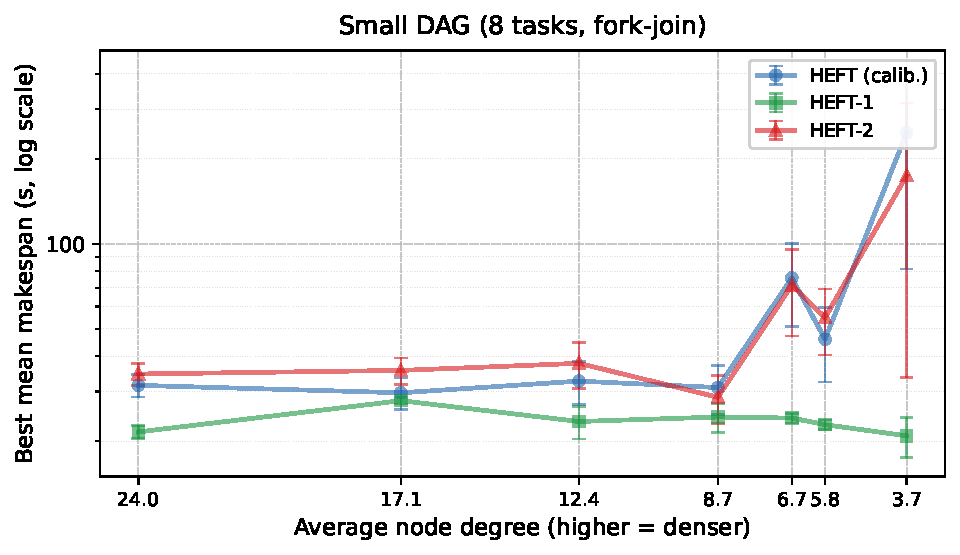
\includegraphics[width=0.88\textwidth]{density_small.pdf}
\caption{Best-routing makespan vs.\ avg degree --- Small DAG (8 tasks, fork-join). Error bars show $\pm$1\,std over 30 seeds.}
\end{figure}

\begin{figure}[H]\centering
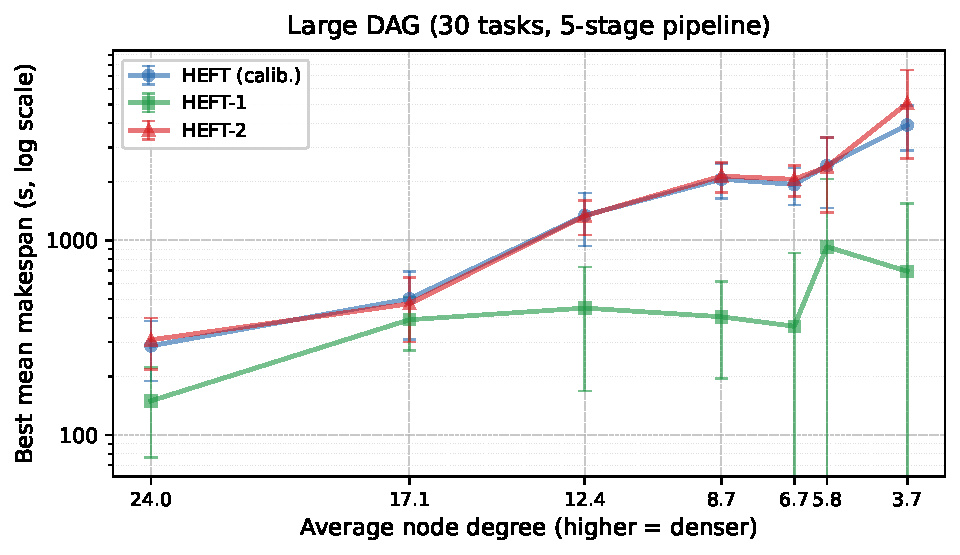
\includegraphics[width=0.88\textwidth]{density_large.pdf}
\caption{Best-routing makespan vs.\ avg degree --- Large DAG (30 tasks, 5-stage pipeline). Error bars show $\pm$1\,std over 30 seeds.}
\end{figure}

\section{Additional Metrics vs.\ Density (Large DAG)}

Computed at the best routing scheme per (density, scheduler) cell.

\begin{figure}[H]\centering
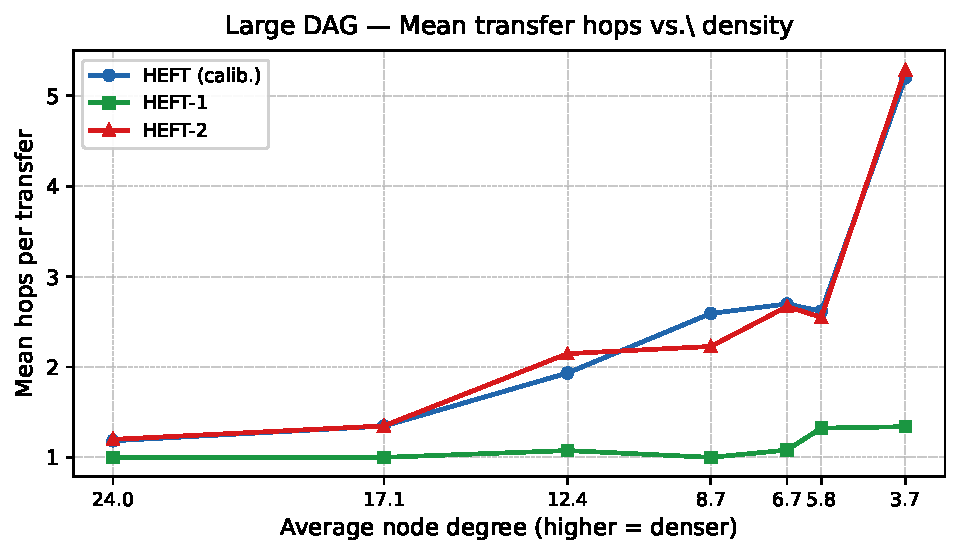
\includegraphics[width=0.88\textwidth]{density_hops_large.pdf}
\caption{Mean hops per transfer. Values $>1$ indicate multi-hop paths.}
\end{figure}

\begin{figure}[H]\centering
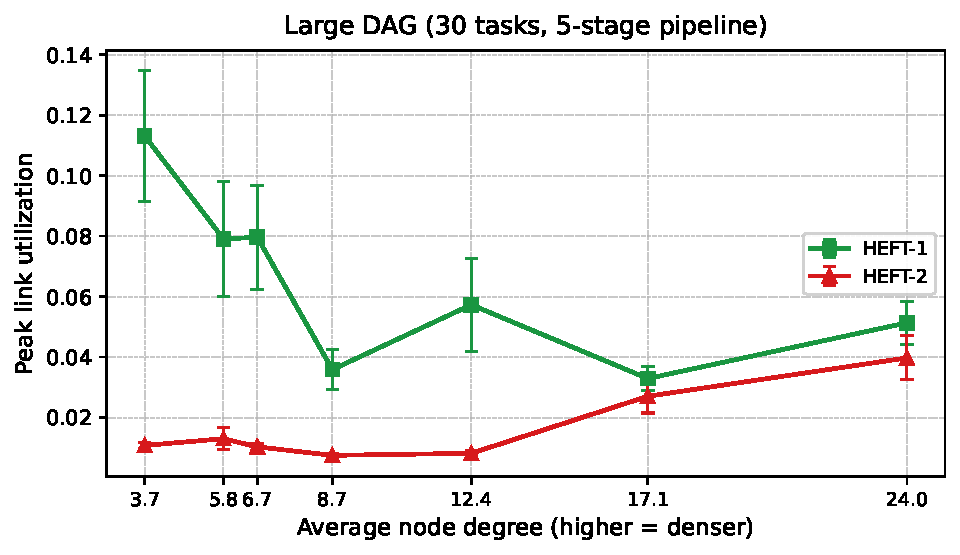
\includegraphics[width=0.88\textwidth]{density_plu_large.pdf}
\caption{Peak link utilization (max over all links). High values indicate congestion hotspots.}
\end{figure}

\begin{figure}[H]\centering
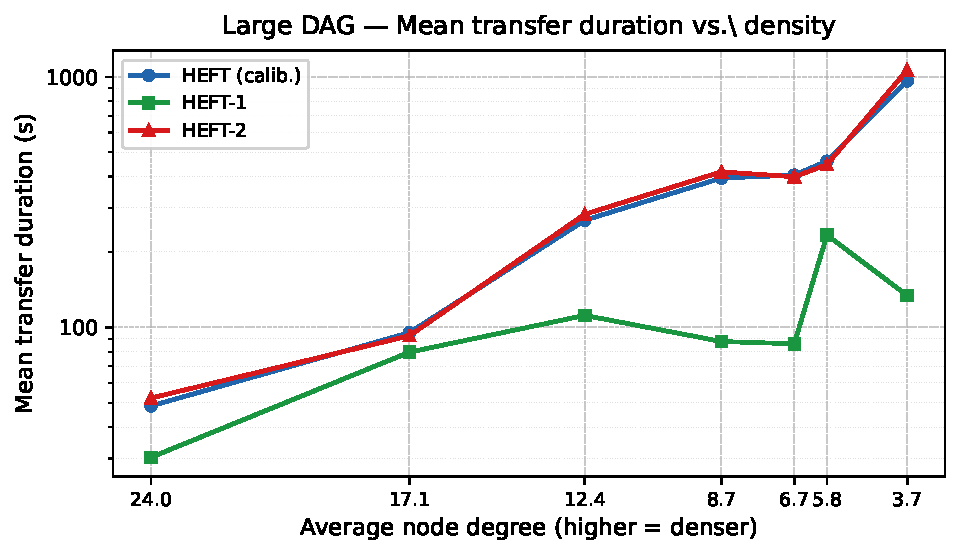
\includegraphics[width=0.88\textwidth]{density_xd_large.pdf}
\caption{Mean transfer duration (s, log scale). Tracks makespan closely.}
\end{figure}

\section{Best Routing per Density and Scheduler}

\subsection{Small DAG (8 tasks)}
\begin{table}[H]\centering\small
\begin{tabular}{l r r@{\,}l@{$\pm$}l@{\,}r r@{\,}l@{$\pm$}l@{\,}r r@{\,}l@{$\pm$}l@{\,}r}
\toprule
\textbf{Dens.} & \textbf{Deg.} & \multicolumn{4}{c}{\textbf{HEFT (calib.)}} & \multicolumn{4}{c}{\textbf{HEFT-1}} & \multicolumn{4}{c}{\textbf{HEFT-2}} \\
\cmidrule(lr){3-6}\cmidrule(lr){7-10}\cmidrule(lr){11-14}
& & \textbf{Rt} & \multicolumn{2}{c}{\textbf{ms (s)}} & \textbf{H/PLU} & \textbf{Rt} & \multicolumn{2}{c}{\textbf{ms (s)}} & \textbf{H/PLU} & \textbf{Rt} & \multicolumn{2}{c}{\textbf{ms (s)}} & \textbf{H/PLU} \\
\midrule
  L150 & 24.0 & S & 31.584 & 7.768 & 1.1/0.20 & S & 21.594 & 3.096 & 1.0/0.19 & S & 34.633 & 8.195 & 1.1/0.21 \\
  L200 & 17.1 & SH & 29.712 & 10.225 & 1.0/0.20 & S & 27.861 & 2.003 & 1.0/0.16 & SH & 35.664 & 10.197 & 1.0/0.22 \\
  L250 & 12.4 & S & 32.688 & 15.283 & 1.1/0.19 & S & 23.513 & 8.325 & 1.0/0.17 & S & 37.796 & 18.701 & 1.2/0.18 \\
  L300 & 8.7 & SH & 31.009 & 16.365 & 1.3/0.18 & SH & 24.388 & 7.755 & 1.0/0.18 & SH & 28.641 & 14.774 & 1.2/0.17 \\
  L350 & 6.7 & SH & 75.816 & 66.186 & 1.8/0.17 & SH & 24.179 & 2.499 & 1.0/0.22 & SH & 71.486 & 65.031 & 1.7/0.17 \\
  L400 & 5.8 & SH & 45.980 & 36.165 & 1.3/0.18 & S & 22.909 & 2.360 & 1.0/0.24 & SH & 54.861 & 38.762 & 1.4/0.20 \\
  L500 & 3.7 & S & 247.261 & 443.820 & 2.1/0.17 & S & \win{20.926} & 9.049 & 1.0/0.29 & GS & 174.510 & 377.184 & 1.8/0.21 \\
\bottomrule\end{tabular}
\caption{Small DAG (8 tasks) --- best routing per (density, scheduler). ms = mean $\pm$ std makespan (s); H = mean hops; PLU = peak link util. \win{Bold green}: overall best.}
\end{table}

\subsection{Large DAG (30 tasks)}
\begin{table}[H]\centering\small
\begin{tabular}{l r r@{\,}l@{$\pm$}l@{\,}r r@{\,}l@{$\pm$}l@{\,}r r@{\,}l@{$\pm$}l@{\,}r}
\toprule
\textbf{Dens.} & \textbf{Deg.} & \multicolumn{4}{c}{\textbf{HEFT (calib.)}} & \multicolumn{4}{c}{\textbf{HEFT-1}} & \multicolumn{4}{c}{\textbf{HEFT-2}} \\
\cmidrule(lr){3-6}\cmidrule(lr){7-10}\cmidrule(lr){11-14}
& & \textbf{Rt} & \multicolumn{2}{c}{\textbf{ms (s)}} & \textbf{H/PLU} & \textbf{Rt} & \multicolumn{2}{c}{\textbf{ms (s)}} & \textbf{H/PLU} & \textbf{Rt} & \multicolumn{2}{c}{\textbf{ms (s)}} & \textbf{H/PLU} \\
\midrule
  L150 & 24.0 & SH & 287.323 & 97.615 & 1.2/0.04 & SH & \win{149.899} & 73.082 & 1.0/0.05 & SH & 308.494 & 90.917 & 1.2/0.04 \\
  L200 & 17.1 & SH & 501.174 & 191.253 & 1.3/0.03 & SH & 391.400 & 119.854 & 1.0/0.03 & SH & 472.856 & 171.599 & 1.3/0.03 \\
  L250 & 12.4 & SH & 1344.549 & 408.317 & 1.9/0.01 & S & 449.477 & 280.738 & 1.1/0.06 & S & 1336.595 & 270.894 & 2.1/0.01 \\
  L300 & 8.7 & S & 2063.615 & 416.010 & 2.6/0.01 & SH & 405.276 & 209.779 & 1.0/0.04 & SH & 2140.430 & 381.959 & 2.2/0.01 \\
  L350 & 6.7 & S & 1939.103 & 415.676 & 2.7/0.01 & SH & 362.181 & 498.494 & 1.1/0.09 & S & 2060.780 & 374.358 & 2.7/0.01 \\
  L400 & 5.8 & SH & 2426.675 & 956.493 & 2.6/0.01 & W & 927.487 & 1143.686 & 1.3/0.09 & SH & 2388.566 & 999.895 & 2.6/0.02 \\
  L500 & 3.7 & S & 3914.460 & 1026.203 & 5.2/0.01 & GSD-D & 694.194 & 848.372 & 1.3/0.09 & GSD-D & 5068.567 & 2436.577 & 5.3/0.01 \\
\bottomrule\end{tabular}
\caption{Large DAG (30 tasks) --- best routing per (density, scheduler). ms = mean $\pm$ std makespan (s); H = mean hops; PLU = peak link util. \win{Bold green}: overall best.}
\end{table}

\section{Full Results Tables}

Mean $\pm$ std makespan (s), mean hops, peak link util over 30 seeds. \win{Bold green}: overall best for density+DAG. \bad{Red}: worst per scheduler column.

\subsection{L150 (avg.\ degree 24.0) --- Small DAG (8 tasks)}
\begin{table}[H]\centering\small
\begin{tabular}{l r@{$\pm$}l r r r@{$\pm$}l r r r@{$\pm$}l r r}
\toprule
\textbf{Route} & \multicolumn{4}{c}{\textbf{HEFT}} & \multicolumn{4}{c}{\textbf{HEFT-1}} & \multicolumn{4}{c}{\textbf{HEFT-2}} \\
\cmidrule(lr){2-5}\cmidrule(lr){6-9}\cmidrule(lr){10-13}
& \multicolumn{2}{c}{\textbf{ms (s)}} & \textbf{H} & \textbf{PLU}& \multicolumn{2}{c}{\textbf{ms (s)}} & \textbf{H} & \textbf{PLU}& \multicolumn{2}{c}{\textbf{ms (s)}} & \textbf{H} & \textbf{PLU} \\
\midrule
  W & 494.056 & 395.759 & 4.0 & 0.017 & 43.651 & 21.247 & 2.2 & 0.108 & 520.163 & 438.020 & 4.3 & 0.018 \\
  S & 31.584 & 7.768 & 1.1 & 0.198 & \win{21.594} & 3.096 & 1.0 & 0.187 & 34.633 & 8.195 & 1.1 & 0.211 \\
  SH & 36.964 & 9.209 & 1.0 & 0.208 & 21.956 & 3.415 & 1.0 & 0.187 & 35.639 & 9.482 & 1.0 & 0.204 \\
  GO & 536.541 & 264.293 & 3.6 & 0.044 & 242.145 & 16.366 & 3.8 & 0.059 & 612.818 & 246.323 & 3.6 & 0.036 \\
  GS & 589.876 & 180.502 & 3.7 & 0.040 & \bad{286.759} & 82.371 & 3.4 & 0.059 & 562.633 & 188.999 & 3.8 & 0.042 \\
  GSD & \bad{640.136} & 286.646 & 4.3 & 0.038 & 286.083 & 111.159 & 2.0 & 0.056 & \bad{639.593} & 293.681 & 4.4 & 0.040 \\
  GSD-D & 414.070 & 86.841 & 4.7 & 0.058 & 144.089 & 33.607 & 2.0 & 0.095 & 409.654 & 120.001 & 4.9 & 0.063 \\
\bottomrule\end{tabular}
\caption{L150 ($L=150$\,m) --- Small DAG (8 tasks). ms = mean$\pm$std; H = mean hops; PLU = peak link util.}
\end{table}

\subsection{L200 (avg.\ degree 17.1) --- Small DAG (8 tasks)}
\begin{table}[H]\centering\small
\begin{tabular}{l r@{$\pm$}l r r r@{$\pm$}l r r r@{$\pm$}l r r}
\toprule
\textbf{Route} & \multicolumn{4}{c}{\textbf{HEFT}} & \multicolumn{4}{c}{\textbf{HEFT-1}} & \multicolumn{4}{c}{\textbf{HEFT-2}} \\
\cmidrule(lr){2-5}\cmidrule(lr){6-9}\cmidrule(lr){10-13}
& \multicolumn{2}{c}{\textbf{ms (s)}} & \textbf{H} & \textbf{PLU}& \multicolumn{2}{c}{\textbf{ms (s)}} & \textbf{H} & \textbf{PLU}& \multicolumn{2}{c}{\textbf{ms (s)}} & \textbf{H} & \textbf{PLU} \\
\midrule
  W & 517.000 & 532.748 & 3.8 & 0.076 & 43.892 & 24.800 & 1.9 & 0.127 & 460.683 & 495.829 & 3.6 & 0.083 \\
  S & 38.313 & 21.088 & 1.3 & 0.158 & \win{27.861} & 2.003 & 1.0 & 0.164 & 38.134 & 19.738 & 1.3 & 0.171 \\
  SH & 29.712 & 10.225 & 1.0 & 0.200 & 28.909 & 2.398 & 1.0 & 0.190 & 35.664 & 10.197 & 1.0 & 0.217 \\
  GO & 872.239 & 1243.295 & 3.5 & 0.066 & 411.368 & 399.410 & 3.1 & 0.068 & \bad{1184.579} & 1483.464 & 3.5 & 0.062 \\
  GS & \bad{1088.416} & 1411.899 & 3.3 & 0.060 & \bad{489.974} & 469.038 & 3.1 & 0.057 & 888.119 & 1236.443 & 3.4 & 0.067 \\
  GSD & 990.931 & 1329.407 & 3.0 & 0.052 & 483.804 & 470.428 & 2.2 & 0.053 & 936.577 & 1214.990 & 4.7 & 0.053 \\
  GSD-D & 459.646 & 725.769 & 3.9 & 0.115 & 229.148 & 212.339 & 1.8 & 0.109 & 830.506 & 1079.304 & 3.8 & 0.091 \\
\bottomrule\end{tabular}
\caption{L200 ($L=200$\,m) --- Small DAG (8 tasks). ms = mean$\pm$std; H = mean hops; PLU = peak link util.}
\end{table}

\subsection{L250 (avg.\ degree 12.4) --- Small DAG (8 tasks)}
\begin{table}[H]\centering\small
\begin{tabular}{l r@{$\pm$}l r r r@{$\pm$}l r r r@{$\pm$}l r r}
\toprule
\textbf{Route} & \multicolumn{4}{c}{\textbf{HEFT}} & \multicolumn{4}{c}{\textbf{HEFT-1}} & \multicolumn{4}{c}{\textbf{HEFT-2}} \\
\cmidrule(lr){2-5}\cmidrule(lr){6-9}\cmidrule(lr){10-13}
& \multicolumn{2}{c}{\textbf{ms (s)}} & \textbf{H} & \textbf{PLU}& \multicolumn{2}{c}{\textbf{ms (s)}} & \textbf{H} & \textbf{PLU}& \multicolumn{2}{c}{\textbf{ms (s)}} & \textbf{H} & \textbf{PLU} \\
\midrule
  W & \bad{609.587} & 762.389 & 2.8 & 0.116 & 29.521 & 17.147 & 1.1 & 0.165 & 546.569 & 737.574 & 2.7 & 0.116 \\
  S & 32.688 & 15.283 & 1.1 & 0.192 & \win{23.513} & 8.325 & 1.0 & 0.170 & 37.796 & 18.701 & 1.2 & 0.180 \\
  SH & 41.687 & 19.984 & 1.3 & 0.172 & 25.843 & 9.323 & 1.0 & 0.174 & 38.534 & 19.627 & 1.2 & 0.170 \\
  GO & 596.181 & 852.593 & 2.9 & 0.086 & 106.264 & 96.645 & 2.5 & 0.111 & 405.795 & 704.200 & 2.7 & 0.101 \\
  GS & 250.967 & 285.347 & 2.7 & 0.106 & 91.428 & 81.701 & 2.4 & 0.119 & 314.147 & 287.965 & 2.8 & 0.093 \\
  GSD & 468.916 & 538.406 & 2.6 & 0.088 & \bad{118.211} & 97.194 & 1.1 & 0.115 & \bad{629.508} & 591.167 & 3.1 & 0.075 \\
  GSD-D & 190.333 & 149.557 & 2.5 & 0.116 & 84.703 & 76.800 & 1.1 & 0.132 & 209.977 & 177.291 & 3.1 & 0.101 \\
\bottomrule\end{tabular}
\caption{L250 ($L=250$\,m) --- Small DAG (8 tasks). ms = mean$\pm$std; H = mean hops; PLU = peak link util.}
\end{table}

\subsection{L300 (avg.\ degree 8.7) --- Small DAG (8 tasks)}
\begin{table}[H]\centering\small
\begin{tabular}{l r@{$\pm$}l r r r@{$\pm$}l r r r@{$\pm$}l r r}
\toprule
\textbf{Route} & \multicolumn{4}{c}{\textbf{HEFT}} & \multicolumn{4}{c}{\textbf{HEFT-1}} & \multicolumn{4}{c}{\textbf{HEFT-2}} \\
\cmidrule(lr){2-5}\cmidrule(lr){6-9}\cmidrule(lr){10-13}
& \multicolumn{2}{c}{\textbf{ms (s)}} & \textbf{H} & \textbf{PLU}& \multicolumn{2}{c}{\textbf{ms (s)}} & \textbf{H} & \textbf{PLU}& \multicolumn{2}{c}{\textbf{ms (s)}} & \textbf{H} & \textbf{PLU} \\
\midrule
  W & 847.135 & 960.462 & 3.4 & 0.106 & 28.512 & 8.633 & 1.1 & 0.178 & 720.078 & 934.033 & 3.1 & 0.120 \\
  S & 34.708 & 17.786 & 1.4 & 0.166 & 26.982 & 8.666 & 1.0 & 0.181 & 33.490 & 17.405 & 1.3 & 0.168 \\
  SH & 31.009 & 16.365 & 1.3 & 0.181 & \win{24.388} & 7.755 & 1.0 & 0.175 & 28.641 & 14.774 & 1.2 & 0.171 \\
  GO & \bad{1067.400} & 1275.536 & 2.5 & 0.072 & \bad{151.303} & 139.010 & 2.3 & 0.112 & 730.413 & 1128.691 & 2.3 & 0.083 \\
  GS & 916.827 & 1177.032 & 2.6 & 0.071 & 129.153 & 136.506 & 2.1 & 0.122 & 576.451 & 891.467 & 2.3 & 0.083 \\
  GSD & 361.737 & 647.347 & 2.1 & 0.116 & 109.158 & 128.730 & 1.2 & 0.133 & \bad{871.740} & 845.597 & 3.8 & 0.073 \\
  GSD-D & 476.092 & 792.718 & 2.4 & 0.127 & 116.086 & 115.703 & 1.3 & 0.156 & 475.722 & 702.279 & 2.7 & 0.119 \\
\bottomrule\end{tabular}
\caption{L300 ($L=300$\,m) --- Small DAG (8 tasks). ms = mean$\pm$std; H = mean hops; PLU = peak link util.}
\end{table}

\subsection{L350 (avg.\ degree 6.7) --- Small DAG (8 tasks)}
\begin{table}[H]\centering\small
\begin{tabular}{l r@{$\pm$}l r r r@{$\pm$}l r r r@{$\pm$}l r r}
\toprule
\textbf{Route} & \multicolumn{4}{c}{\textbf{HEFT}} & \multicolumn{4}{c}{\textbf{HEFT-1}} & \multicolumn{4}{c}{\textbf{HEFT-2}} \\
\cmidrule(lr){2-5}\cmidrule(lr){6-9}\cmidrule(lr){10-13}
& \multicolumn{2}{c}{\textbf{ms (s)}} & \textbf{H} & \textbf{PLU}& \multicolumn{2}{c}{\textbf{ms (s)}} & \textbf{H} & \textbf{PLU}& \multicolumn{2}{c}{\textbf{ms (s)}} & \textbf{H} & \textbf{PLU} \\
\midrule
  W & 692.048 & 1028.635 & 2.8 & 0.111 & 24.745 & 6.684 & 1.1 & 0.233 & 985.791 & 1112.765 & 3.4 & 0.091 \\
  S & 414.203 & 830.766 & 2.2 & 0.141 & 25.020 & 5.279 & 1.1 & 0.211 & 331.440 & 761.427 & 1.9 & 0.153 \\
  SH & 75.816 & 66.186 & 1.8 & 0.169 & \win{24.179} & 2.499 & 1.0 & 0.217 & 71.486 & 65.031 & 1.7 & 0.167 \\
  GO & \bad{1115.620} & 1443.721 & 2.3 & 0.094 & 40.942 & 23.034 & 1.6 & 0.189 & \bad{1312.776} & 1483.877 & 2.5 & 0.084 \\
  GS & 1015.965 & 1413.352 & 2.2 & 0.099 & 52.288 & 22.199 & 1.8 & 0.170 & 625.956 & 1197.779 & 1.9 & 0.115 \\
  GSD & 336.893 & 896.596 & 1.9 & 0.123 & \bad{54.115} & 21.714 & 1.2 & 0.168 & 1215.382 & 1466.386 & 3.2 & 0.088 \\
  GSD-D & 1113.997 & 1444.052 & 3.0 & 0.103 & 39.763 & 23.657 & 1.1 & 0.223 & 917.628 & 1373.200 & 2.7 & 0.113 \\
\bottomrule\end{tabular}
\caption{L350 ($L=350$\,m) --- Small DAG (8 tasks). ms = mean$\pm$std; H = mean hops; PLU = peak link util.}
\end{table}

\subsection{L400 (avg.\ degree 5.8) --- Small DAG (8 tasks)}
\begin{table}[H]\centering\small
\begin{tabular}{l r@{$\pm$}l r r r@{$\pm$}l r r r@{$\pm$}l r r}
\toprule
\textbf{Route} & \multicolumn{4}{c}{\textbf{HEFT}} & \multicolumn{4}{c}{\textbf{HEFT-1}} & \multicolumn{4}{c}{\textbf{HEFT-2}} \\
\cmidrule(lr){2-5}\cmidrule(lr){6-9}\cmidrule(lr){10-13}
& \multicolumn{2}{c}{\textbf{ms (s)}} & \textbf{H} & \textbf{PLU}& \multicolumn{2}{c}{\textbf{ms (s)}} & \textbf{H} & \textbf{PLU}& \multicolumn{2}{c}{\textbf{ms (s)}} & \textbf{H} & \textbf{PLU} \\
\midrule
  W & \bad{837.123} & 1083.421 & 3.1 & 0.138 & 29.321 & 8.893 & 1.3 & 0.209 & \bad{689.413} & 1030.510 & 2.7 & 0.144 \\
  S & 615.176 & 994.768 & 2.6 & 0.139 & \win{22.909} & 2.360 & 1.0 & 0.238 & 615.634 & 994.487 & 2.6 & 0.149 \\
  SH & 45.980 & 36.165 & 1.3 & 0.181 & 23.741 & 2.347 & 1.0 & 0.231 & 54.861 & 38.762 & 1.4 & 0.203 \\
  GO & 503.103 & 883.794 & 2.7 & 0.108 & 207.313 & 170.499 & 2.1 & 0.118 & 512.725 & 879.083 & 2.8 & 0.104 \\
  GS & 440.730 & 819.410 & 2.6 & 0.106 & \bad{255.294} & 138.328 & 2.5 & 0.086 & 384.038 & 743.134 & 2.6 & 0.119 \\
  GSD & 437.806 & 820.867 & 2.8 & 0.122 & 243.985 & 155.792 & 1.3 & 0.086 & 592.820 & 924.366 & 3.2 & 0.109 \\
  GSD-D & 423.879 & 825.860 & 2.3 & 0.138 & 117.097 & 115.572 & 1.1 & 0.182 & 433.288 & 822.376 & 2.7 & 0.137 \\
\bottomrule\end{tabular}
\caption{L400 ($L=400$\,m) --- Small DAG (8 tasks). ms = mean$\pm$std; H = mean hops; PLU = peak link util.}
\end{table}

\subsection{L500 (avg.\ degree 3.7) --- Small DAG (8 tasks)}
\begin{table}[H]\centering\small
\begin{tabular}{l r@{$\pm$}l r r r@{$\pm$}l r r r@{$\pm$}l r r}
\toprule
\textbf{Route} & \multicolumn{4}{c}{\textbf{HEFT}} & \multicolumn{4}{c}{\textbf{HEFT-1}} & \multicolumn{4}{c}{\textbf{HEFT-2}} \\
\cmidrule(lr){2-5}\cmidrule(lr){6-9}\cmidrule(lr){10-13}
& \multicolumn{2}{c}{\textbf{ms (s)}} & \textbf{H} & \textbf{PLU}& \multicolumn{2}{c}{\textbf{ms (s)}} & \textbf{H} & \textbf{PLU}& \multicolumn{2}{c}{\textbf{ms (s)}} & \textbf{H} & \textbf{PLU} \\
\midrule
  W & 356.336 & 508.470 & 2.9 & 0.168 & 21.669 & 8.205 & 1.0 & 0.282 & 210.881 & 413.512 & 2.0 & 0.197 \\
  S & 247.261 & 443.820 & 2.1 & 0.174 & \win{20.926} & 9.049 & 1.0 & 0.286 & 392.711 & 523.049 & 2.9 & 0.149 \\
  SH & \bad{501.809} & 549.817 & 3.4 & 0.121 & 23.151 & 8.785 & 1.0 & 0.297 & \bad{465.443} & 543.565 & 3.2 & 0.131 \\
  GO & \bad{501.795} & 549.830 & 3.5 & 0.134 & 22.127 & 7.384 & 1.0 & 0.277 & \bad{465.438} & 543.568 & 3.5 & 0.135 \\
  GS & 429.050 & 534.708 & 3.2 & 0.167 & 21.384 & 8.354 & 1.0 & 0.282 & 174.510 & 377.184 & 1.8 & 0.211 \\
  GSD & 392.711 & 523.049 & 3.1 & 0.149 & \bad{32.377} & 21.924 & 1.0 & 0.208 & 356.363 & 508.452 & 2.8 & 0.141 \\
  GSD-D & 318.912 & 491.322 & 2.6 & 0.173 & 21.863 & 8.663 & 1.0 & 0.312 & 318.765 & 491.411 & 2.6 & 0.198 \\
\bottomrule\end{tabular}
\caption{L500 ($L=500$\,m) --- Small DAG (8 tasks). ms = mean$\pm$std; H = mean hops; PLU = peak link util.}
\end{table}

\subsection{L150 (avg.\ degree 24.0) --- Large DAG (30 tasks)}
\begin{table}[H]\centering\small
\begin{tabular}{l r@{$\pm$}l r r r@{$\pm$}l r r r@{$\pm$}l r r}
\toprule
\textbf{Route} & \multicolumn{4}{c}{\textbf{HEFT}} & \multicolumn{4}{c}{\textbf{HEFT-1}} & \multicolumn{4}{c}{\textbf{HEFT-2}} \\
\cmidrule(lr){2-5}\cmidrule(lr){6-9}\cmidrule(lr){10-13}
& \multicolumn{2}{c}{\textbf{ms (s)}} & \textbf{H} & \textbf{PLU}& \multicolumn{2}{c}{\textbf{ms (s)}} & \textbf{H} & \textbf{PLU}& \multicolumn{2}{c}{\textbf{ms (s)}} & \textbf{H} & \textbf{PLU} \\
\midrule
  W & 1530.829 & 223.415 & 5.5 & 0.007 & 542.056 & 310.803 & 2.5 & 0.020 & 1504.689 & 235.408 & 5.6 & 0.007 \\
  S & 715.431 & 279.178 & 1.7 & 0.020 & 198.784 & 101.554 & 1.2 & 0.047 & 675.535 & 308.317 & 1.7 & 0.022 \\
  SH & 287.323 & 97.615 & 1.2 & 0.041 & \win{149.899} & 73.082 & 1.0 & 0.049 & 308.494 & 90.917 & 1.2 & 0.041 \\
  GO & 3540.427 & 676.048 & 3.8 & 0.008 & 2117.429 & 762.023 & 3.5 & 0.021 & 3383.308 & 672.062 & 3.8 & 0.009 \\
  GS & \bad{3567.396} & 735.216 & 3.9 & 0.008 & \bad{2501.810} & 691.324 & 3.7 & 0.016 & \bad{3589.212} & 705.323 & 3.8 & 0.008 \\
  GSD & 3256.273 & 422.823 & 5.5 & 0.008 & 2192.774 & 755.378 & 2.5 & 0.018 & 3309.441 & 386.379 & 5.5 & 0.008 \\
  GSD-D & 2601.980 & 292.511 & 5.4 & 0.010 & 1805.307 & 545.149 & 2.6 & 0.021 & 2568.484 & 279.133 & 5.5 & 0.011 \\
\bottomrule\end{tabular}
\caption{L150 ($L=150$\,m) --- Large DAG (30 tasks). ms = mean$\pm$std; H = mean hops; PLU = peak link util.}
\end{table}

\subsection{L200 (avg.\ degree 17.1) --- Large DAG (30 tasks)}
\begin{table}[H]\centering\small
\begin{tabular}{l r@{$\pm$}l r r r@{$\pm$}l r r r@{$\pm$}l r r}
\toprule
\textbf{Route} & \multicolumn{4}{c}{\textbf{HEFT}} & \multicolumn{4}{c}{\textbf{HEFT-1}} & \multicolumn{4}{c}{\textbf{HEFT-2}} \\
\cmidrule(lr){2-5}\cmidrule(lr){6-9}\cmidrule(lr){10-13}
& \multicolumn{2}{c}{\textbf{ms (s)}} & \textbf{H} & \textbf{PLU}& \multicolumn{2}{c}{\textbf{ms (s)}} & \textbf{H} & \textbf{PLU}& \multicolumn{2}{c}{\textbf{ms (s)}} & \textbf{H} & \textbf{PLU} \\
\midrule
  W & 1943.409 & 388.855 & 5.7 & 0.007 & 1079.533 & 492.574 & 2.5 & 0.016 & 1822.756 & 382.398 & 5.4 & 0.007 \\
  S & 831.126 & 115.776 & 1.8 & 0.016 & 410.010 & 137.880 & 1.0 & 0.030 & 860.765 & 153.697 & 1.8 & 0.015 \\
  SH & 501.174 & 191.253 & 1.3 & 0.025 & \win{391.400} & 119.854 & 1.0 & 0.030 & 472.856 & 171.599 & 1.3 & 0.027 \\
  GO & \bad{4049.688} & 600.687 & 3.7 & 0.010 & 3425.021 & 1261.481 & 3.6 & 0.015 & \bad{4131.985} & 457.422 & 3.7 & 0.010 \\
  GS & 3973.898 & 815.731 & 3.7 & 0.010 & \bad{4263.847} & 2151.727 & 3.5 & 0.011 & 3671.203 & 731.394 & 3.7 & 0.010 \\
  GSD & 3531.402 & 676.131 & 5.6 & 0.010 & 3902.399 & 2000.261 & 2.5 & 0.013 & 3652.316 & 735.637 & 5.7 & 0.010 \\
  GSD-D & 3131.900 & 861.145 & 5.5 & 0.013 & 2520.026 & 472.214 & 2.3 & 0.018 & 2981.828 & 838.339 & 5.7 & 0.013 \\
\bottomrule\end{tabular}
\caption{L200 ($L=200$\,m) --- Large DAG (30 tasks). ms = mean$\pm$std; H = mean hops; PLU = peak link util.}
\end{table}

\subsection{L250 (avg.\ degree 12.4) --- Large DAG (30 tasks)}
\begin{table}[H]\centering\small
\begin{tabular}{l r@{$\pm$}l r r r@{$\pm$}l r r r@{$\pm$}l r r}
\toprule
\textbf{Route} & \multicolumn{4}{c}{\textbf{HEFT}} & \multicolumn{4}{c}{\textbf{HEFT-1}} & \multicolumn{4}{c}{\textbf{HEFT-2}} \\
\cmidrule(lr){2-5}\cmidrule(lr){6-9}\cmidrule(lr){10-13}
& \multicolumn{2}{c}{\textbf{ms (s)}} & \textbf{H} & \textbf{PLU}& \multicolumn{2}{c}{\textbf{ms (s)}} & \textbf{H} & \textbf{PLU}& \multicolumn{2}{c}{\textbf{ms (s)}} & \textbf{H} & \textbf{PLU} \\
\midrule
  W & 1812.396 & 310.729 & 4.8 & 0.009 & 626.690 & 278.479 & 1.9 & 0.032 & 1852.661 & 281.293 & 4.7 & 0.009 \\
  S & 1357.554 & 260.999 & 2.1 & 0.008 & \win{449.477} & 280.738 & 1.1 & 0.056 & 1336.595 & 270.894 & 2.1 & 0.009 \\
  SH & 1344.549 & 408.317 & 1.9 & 0.010 & 559.928 & 276.236 & 1.0 & 0.044 & 1361.136 & 392.196 & 1.9 & 0.010 \\
  GO & \bad{3063.776} & 440.036 & 3.7 & 0.009 & 1262.239 & 297.262 & 3.1 & 0.029 & 2986.991 & 407.257 & 3.7 & 0.008 \\
  GS & 3048.733 & 495.837 & 3.4 & 0.007 & 1820.238 & 996.768 & 3.0 & 0.025 & \bad{3023.702} & 470.928 & 3.5 & 0.008 \\
  GSD & 2530.877 & 381.148 & 4.8 & 0.008 & \bad{1835.618} & 882.414 & 2.0 & 0.019 & 2602.391 & 333.341 & 4.8 & 0.008 \\
  GSD-D & 1951.639 & 313.426 & 4.7 & 0.011 & 1226.291 & 669.369 & 1.9 & 0.029 & 1924.656 & 320.437 & 4.7 & 0.011 \\
\bottomrule\end{tabular}
\caption{L250 ($L=250$\,m) --- Large DAG (30 tasks). ms = mean$\pm$std; H = mean hops; PLU = peak link util.}
\end{table}

\subsection{L300 (avg.\ degree 8.7) --- Large DAG (30 tasks)}
\begin{table}[H]\centering\small
\begin{tabular}{l r@{$\pm$}l r r r@{$\pm$}l r r r@{$\pm$}l r r}
\toprule
\textbf{Route} & \multicolumn{4}{c}{\textbf{HEFT}} & \multicolumn{4}{c}{\textbf{HEFT-1}} & \multicolumn{4}{c}{\textbf{HEFT-2}} \\
\cmidrule(lr){2-5}\cmidrule(lr){6-9}\cmidrule(lr){10-13}
& \multicolumn{2}{c}{\textbf{ms (s)}} & \textbf{H} & \textbf{PLU}& \multicolumn{2}{c}{\textbf{ms (s)}} & \textbf{H} & \textbf{PLU}& \multicolumn{2}{c}{\textbf{ms (s)}} & \textbf{H} & \textbf{PLU} \\
\midrule
  W & 2639.992 & 634.022 & 4.9 & 0.006 & 809.067 & 640.877 & 1.9 & 0.047 & 2726.267 & 613.490 & 5.5 & 0.006 \\
  S & 2063.615 & 416.010 & 2.6 & 0.008 & 428.149 & 248.501 & 1.1 & 0.041 & 2156.510 & 308.769 & 2.7 & 0.007 \\
  SH & 2233.182 & 362.908 & 2.4 & 0.007 & \win{405.276} & 209.779 & 1.0 & 0.040 & 2140.430 & 381.959 & 2.2 & 0.007 \\
  GO & 2810.638 & 419.397 & 4.0 & 0.008 & 1078.668 & 370.577 & 1.9 & 0.033 & \bad{2859.602} & 427.744 & 4.0 & 0.008 \\
  GS & \bad{2822.218} & 476.802 & 3.9 & 0.009 & 1027.168 & 284.955 & 1.9 & 0.040 & 2807.280 & 538.642 & 3.9 & 0.009 \\
  GSD & 2769.135 & 245.327 & 5.2 & 0.008 & \bad{1471.472} & 611.280 & 1.9 & 0.022 & 2725.680 & 277.762 & 5.1 & 0.008 \\
  GSD-D & 2740.669 & 815.114 & 5.6 & 0.009 & 998.452 & 50.359 & 1.8 & 0.035 & 2500.433 & 927.019 & 5.2 & 0.010 \\
\bottomrule\end{tabular}
\caption{L300 ($L=300$\,m) --- Large DAG (30 tasks). ms = mean$\pm$std; H = mean hops; PLU = peak link util.}
\end{table}

\subsection{L350 (avg.\ degree 6.7) --- Large DAG (30 tasks)}
\begin{table}[H]\centering\small
\begin{tabular}{l r@{$\pm$}l r r r@{$\pm$}l r r r@{$\pm$}l r r}
\toprule
\textbf{Route} & \multicolumn{4}{c}{\textbf{HEFT}} & \multicolumn{4}{c}{\textbf{HEFT-1}} & \multicolumn{4}{c}{\textbf{HEFT-2}} \\
\cmidrule(lr){2-5}\cmidrule(lr){6-9}\cmidrule(lr){10-13}
& \multicolumn{2}{c}{\textbf{ms (s)}} & \textbf{H} & \textbf{PLU}& \multicolumn{2}{c}{\textbf{ms (s)}} & \textbf{H} & \textbf{PLU}& \multicolumn{2}{c}{\textbf{ms (s)}} & \textbf{H} & \textbf{PLU} \\
\midrule
  W & 2262.481 & 311.049 & 4.3 & 0.009 & 627.582 & 774.416 & 1.3 & 0.093 & 2378.291 & 263.160 & 4.3 & 0.009 \\
  S & 1939.103 & 415.676 & 2.7 & 0.010 & 767.926 & 688.464 & 1.3 & 0.071 & 2060.780 & 374.358 & 2.7 & 0.010 \\
  SH & 2142.480 & 533.937 & 2.5 & 0.011 & \win{362.181} & 498.494 & 1.1 & 0.094 & 2155.497 & 573.914 & 2.6 & 0.011 \\
  GO & 2577.160 & 855.336 & 3.6 & 0.010 & 880.890 & 773.572 & 1.7 & 0.050 & 2406.193 & 763.198 & 3.4 & 0.011 \\
  GS & 2426.125 & 701.306 & 3.9 & 0.010 & \bad{1185.292} & 877.412 & 1.8 & 0.041 & \bad{2483.959} & 651.898 & 3.7 & 0.012 \\
  GSD & \bad{2625.803} & 747.668 & 3.9 & 0.010 & 1028.508 & 734.175 & 1.3 & 0.036 & 2454.205 & 730.232 & 4.0 & 0.010 \\
  GSD-D & 2575.997 & 962.700 & 4.4 & 0.011 & 891.407 & 751.442 & 1.3 & 0.050 & 2353.488 & 909.641 & 4.1 & 0.011 \\
\bottomrule\end{tabular}
\caption{L350 ($L=350$\,m) --- Large DAG (30 tasks). ms = mean$\pm$std; H = mean hops; PLU = peak link util.}
\end{table}

\subsection{L400 (avg.\ degree 5.8) --- Large DAG (30 tasks)}
\begin{table}[H]\centering\small
\begin{tabular}{l r@{$\pm$}l r r r@{$\pm$}l r r r@{$\pm$}l r r}
\toprule
\textbf{Route} & \multicolumn{4}{c}{\textbf{HEFT}} & \multicolumn{4}{c}{\textbf{HEFT-1}} & \multicolumn{4}{c}{\textbf{HEFT-2}} \\
\cmidrule(lr){2-5}\cmidrule(lr){6-9}\cmidrule(lr){10-13}
& \multicolumn{2}{c}{\textbf{ms (s)}} & \textbf{H} & \textbf{PLU}& \multicolumn{2}{c}{\textbf{ms (s)}} & \textbf{H} & \textbf{PLU}& \multicolumn{2}{c}{\textbf{ms (s)}} & \textbf{H} & \textbf{PLU} \\
\midrule
  W & 2844.226 & 831.929 & 3.6 & 0.006 & \win{927.487} & 1143.686 & 1.3 & 0.089 & 2980.537 & 784.045 & 4.4 & 0.006 \\
  S & 2947.258 & 813.232 & 3.8 & 0.007 & 1080.936 & 1271.055 & 1.1 & 0.067 & 2919.019 & 788.194 & 4.3 & 0.007 \\
  SH & 2426.675 & 956.493 & 2.6 & 0.014 & 1252.065 & 1325.088 & 1.1 & 0.064 & 2388.566 & 999.895 & 2.6 & 0.016 \\
  GO & \bad{3331.649} & 276.965 & 4.1 & 0.009 & 1229.818 & 1365.355 & 1.6 & 0.072 & \bad{3336.711} & 299.362 & 4.1 & 0.008 \\
  GS & 3154.020 & 318.127 & 4.7 & 0.009 & 1611.463 & 1425.890 & 1.6 & 0.063 & 3239.241 & 352.323 & 4.5 & 0.009 \\
  GSD & 3209.028 & 430.747 & 3.9 & 0.008 & \bad{1621.605} & 1543.986 & 1.3 & 0.035 & 3065.852 & 370.610 & 4.4 & 0.007 \\
  GSD-D & 3070.476 & 683.704 & 3.8 & 0.008 & 1202.449 & 1351.971 & 1.3 & 0.068 & 3205.536 & 605.676 & 4.3 & 0.007 \\
\bottomrule\end{tabular}
\caption{L400 ($L=400$\,m) --- Large DAG (30 tasks). ms = mean$\pm$std; H = mean hops; PLU = peak link util.}
\end{table}

\subsection{L500 (avg.\ degree 3.7) --- Large DAG (30 tasks)}
\begin{table}[H]\centering\small
\begin{tabular}{l r@{$\pm$}l r r r@{$\pm$}l r r r@{$\pm$}l r r}
\toprule
\textbf{Route} & \multicolumn{4}{c}{\textbf{HEFT}} & \multicolumn{4}{c}{\textbf{HEFT-1}} & \multicolumn{4}{c}{\textbf{HEFT-2}} \\
\cmidrule(lr){2-5}\cmidrule(lr){6-9}\cmidrule(lr){10-13}
& \multicolumn{2}{c}{\textbf{ms (s)}} & \textbf{H} & \textbf{PLU}& \multicolumn{2}{c}{\textbf{ms (s)}} & \textbf{H} & \textbf{PLU}& \multicolumn{2}{c}{\textbf{ms (s)}} & \textbf{H} & \textbf{PLU} \\
\midrule
  W & 5494.190 & 2715.245 & 5.6 & 0.010 & 906.925 & 939.040 & 1.3 & 0.097 & 5732.305 & 2309.919 & 5.0 & 0.011 \\
  S & 3914.460 & 1026.203 & 5.2 & 0.011 & 792.757 & 910.573 & 1.0 & 0.108 & 6166.377 & 2844.477 & 4.9 & 0.011 \\
  SH & \bad{5924.170} & 2780.786 & 5.0 & 0.011 & \bad{1035.847} & 972.957 & 1.1 & 0.091 & \bad{6870.982} & 2578.797 & 4.7 & 0.011 \\
  GO & 4771.168 & 1976.106 & 5.3 & 0.012 & 923.603 & 961.934 & 1.2 & 0.100 & 5773.163 & 2438.199 & 4.6 & 0.013 \\
  GS & 4544.688 & 1723.611 & 5.5 & 0.011 & 860.593 & 945.260 & 1.2 & 0.104 & 5767.751 & 2680.004 & 4.8 & 0.012 \\
  GSD & 5560.900 & 2387.494 & 4.7 & 0.013 & 938.632 & 953.460 & 1.2 & 0.086 & 5386.756 & 1930.721 & 4.7 & 0.013 \\
  GSD-D & 5212.339 & 2344.961 & 5.1 & 0.012 & \win{694.194} & 848.372 & 1.3 & 0.094 & 5068.567 & 2436.577 & 5.3 & 0.012 \\
\bottomrule\end{tabular}
\caption{L500 ($L=500$\,m) --- Large DAG (30 tasks). ms = mean$\pm$std; H = mean hops; PLU = peak link util.}
\end{table}

\section{Analysis}

\subsection{HEFT-1 Dominance Is Robust Across All Densities}

HEFT-1 wins at every density level for both DAGs. For the large DAG, the advantage over calibrated HEFT ranges from $1.9\times$ at L150 to $5.6\times$ at L500. The standard deviations under HEFT and HEFT-2 are large (often $>50$\% of the mean) because csma\_bianchi interference is highly sensitive to the exact traffic pattern, which varies across seeds. HEFT-1's std is much smaller: co-location eliminates most transfers, leaving only compute variance.

\subsection{SH vs.\ S: Density-Dependent Reversal}

Under HEFT-1, SH beats S at L150--L300 for the large DAG (mean-hops = 1.0 for both, confirming co-location). The routing tie-break wins come from how each scheme selects the single hop: SH prefers the nearest (lowest-loss) link, reducing PHY-layer retransmission and thus interference variance. At sparse topologies (L400--L500), fewer 1-hop options exist and S regains the lead by picking the highest-bandwidth available link.

\subsection{Hops, Peak Link Util., and Transfer Duration}

The additional metrics confirm that routing choice under csma\_bianchi is primarily about \emph{which} 1-hop link is used, not multi-hop avoidance:
\begin{itemize}
  \item Mean hops is $\approx 1.0$ for HEFT-1 across all density levels,    confirming that co-located tasks transfer directly to adjacent nodes.
  \item Calibrated HEFT and HEFT-2 use 2--4 hops at high density (L150--L200),    where tasks are spread across many nodes. Multi-hop paths under csma\_bianchi    amplify interference---each relay adds an active transmitter---explaining    the large makespan gap.
  \item Peak link utilization under HEFT-1 is low ($<0.06$) because    co-located tasks do not use links; the few transfers that occur are    short and non-overlapping. Under HEFT/HEFT-2 peak link util can    exceed 0.9, indicating severe bottleneck congestion.
\end{itemize}

\subsection{Reproducing These Results}
\begin{verbatim}
cd ncsim/
python run_random_eval.py                  # ~3500 s (8820 runs)
python compute_interference_metrics.py      # reads traces, ~3 min
python gen_random_network_report.py         # generates tex + plots
cd docs/ && pdflatex random_network_results.tex
\end{verbatim}

\end{document}